\documentclass{sig-alternate-05-2015}

\usepackage{amsmath}
\usepackage{color}
\usepackage{graphicx}
\usepackage{listings}
\usepackage{microtype}
\usepackage{pslatex}
\usepackage{relsize}
\usepackage[pageanchor=false]{hyperref}
\usepackage{balance}

%% Comment out one of these two definitions.
% \newcommand{\todo}[1]{\relax}
\newcommand{\todo}[1]{{\color{red}\bfseries [[#1]]}}

% Single space
\renewcommand{\baselinestretch}{1}


% At least 80% of every float page must be taken up by
% floats; there will be no page with more than 20% white space.
\def\topfraction{.8}
\def\dbltopfraction{\topfraction}
\def\floatpagefraction{\topfraction}     % default .5
\def\dblfloatpagefraction{\topfraction}  % default .5
\def\textfraction{.2}

\lstset{
    language=Java,
    basicstyle=\linespread{0.8}\sf\small,
    aboveskip={1.0\baselineskip},
    belowskip={1.0\baselineskip},
    columns=fixed,
    extendedchars=true,
    breaklines=true,
    tabsize=4,
    prebreak=\raisebox{0ex}[0ex][0ex]{\ensuremath{\hookleftarrow}},
    showtabs=false,
    showspaces=false,
    showstringspaces=false,
    numberstyle=\small,
    stepnumber=1,
    numbersep=10pt,
    captionpos=b,
    escapeinside={\%*}{*)}
}

% \|name| or \mathid{name} denotes identifiers and slots in formulas
\def\|#1|{\mathid{#1}}
\newcommand{\mathid}[1]{\ensuremath{\mathit{#1}}}
% \<name> or \codeid{name} denotes computer code identifiers
\def\<#1>{\codeid{#1}}
\protected\def\codeid#1{\ifmmode{\mbox{\sf{#1}}}\else{\sf #1}\fi}

\begin{document}
\toappear{}

\setlength{\paperheight}{11in}
\setlength{\paperwidth}{8.5in}

\title{Preventing Signedness Errors in Numerical Computations in Java}

\numberofauthors{1} %  in this sample file, there are a *total*
\author{
Christopher A. Mackie\\
       \affaddr{University of Washington Computer Science \& Engineering}\\
       \affaddr{Seattle, WA, USA}\\
       \email{mackic@cs.washington.edu}
}

\maketitle

\section*{ABSTRACT}
We have developed and implemented a type system, the Signedness Type System,
that captures usage of signed and unsigned integers in Java programs. This
type system enables developers to detect errors regarding unsigned integers at
compile time, and guarantees that such errors cannot occur at run time. In a
case study. our type system proved easy to use and detected a previously unknown
bug. Our type system is implemented as the Signedness Checker and will be
available with the Checker Framework (http://CheckerFramework.org/).

% CCS
\begin{CCSXML}
<ccs2012>
<concept>
<concept_id>10002944.10011123.10010577</concept_id>
<concept_desc>General and reference~Reliability</concept_desc>
<concept_significance>500</concept_significance>
</concept>
<concept>
<concept_id>10011007.10010940.10011003.10011004</concept_id>
<concept_desc>Software and its engineering~Software reliability</concept_desc>
<concept_significance>500</concept_significance>
</concept>
</ccs2012>
\end{CCSXML}

\ccsdesc[500]{General and reference~Reliability}
\ccsdesc[500]{Software and its engineering~Software reliability}

\printccsdesc

\keywords{type system, pluggable type checker, java, unsigned numbers}

\section{Problem and Motivation}

Signed integers use the first bit of the machine representation to
encode the sign of a value, whereas unsigned integers use all
bits to represent the magnitude of a value.
Unsigned integers cover a larger range of positive numbers, but cannot represent
negative numbers.
Unsigned integers are useful, so many programming languages support them;
for example, Java 8 introduced utility methods for unsigned
integers~\cite{JDK8UnsignedIntegerArithmetic2012}.  However, they are also
error-prone:  using one where a signed
integer is expected, or performing certain arithmetic operations on unsigned
integers, can lead to unexpected results.

We call an operator ``insensitive'' if it produces a correct signed result
when run on two signed values and a correct unsigned result
when run on two unsigned values.  We call an operator ``sensitive'' if it
produces incorrect results when run on two unsigned values. For such
operations, a programmer must run a different implementation depending on whether
the operands are signed or unsigned.
% See Figure~\ref{fig:operators} for
% an example of insensitive and sensitive operators.

Misuse of unsigned values can be categorized as follows:

\begin{itemize}\itemsep 0pt \parskip 0pt
  \item Using a sensitive operator with unsigned operands.
  \item Mixing signed and unsigned arguments to any operator.
\end{itemize}

The first line of defense against most bugs is the compiler. When the
compiler is unable to catch bugs, it falls on the programmer to identify and
eliminate them, which is prone to human error. The Java compiler
is not helpful in finding bugs related to using unsigned
numbers because Java's unsigned
integers are supported by a library rather than built into Java.

\section{Approach and Uniqueness}

Our approach to detecting and preventing signedness errors is to use a type
system. This has a number of benefits.
%
Compile-time checking permits developers
to catch bugs before they become problems for end-users.
%
Type systems are familiar to programmers, who understand how to use them
and interpret their warning messages.

% Figure appears late in the LaTeX file to prevent it from being placed in
% the first column of the paper.

\begin{figure}[t]
    \centering
    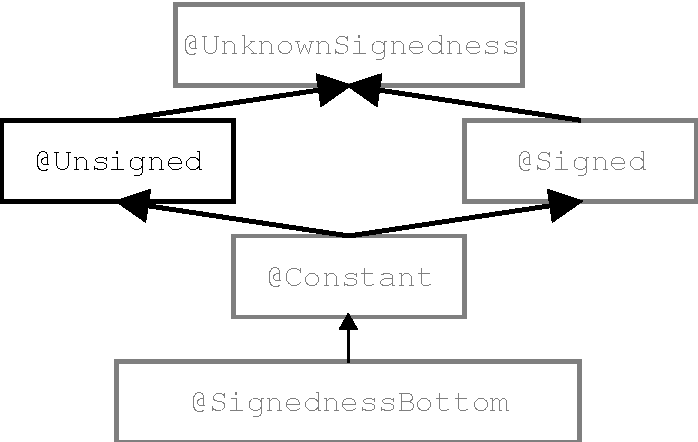
\includegraphics[width=0.35\textwidth]{signedness}
\vspace{-10pt}
    \caption{The type qualifier hierarchy of our type system.
Qualifiers in gray are used internally, and should not be written.}
    \label{fig:type-hierarchy}
\end{figure}

We have defined a type system and implemented it in a tool
called the Signedness Checker.
This type system has five type qualifiers
(Figure~\ref{fig:type-hierarchy}).  Each is written together
with a base type; for example, \<@Unsigned int i> declares a
variable named \<i> of type \<@Unsigned int>.

\begin{itemize}\itemsep 0pt \parskip 0pt
  \item \<@UnknownSignedness> indicates a value for which our tool
   has no estimate.  (This usually leads to a
    warning.)  It is also used for non-numeric
    values, which our tool ignores.
  \item \<@Unsigned> signifies that a value is unsigned.
  \item \<@Signed> signifies that a value is signed.
  \item \<@Constant> is for values known at compile time, such as
    manifest literals.  The programmer might intend to
    use them as signed or as unsigned values.  Even a negative literal may
    be used as a placeholder for a large positive unsigned
    integer.
  \item \<@SignednessBottom> indicates dead code or the \<null> value.
\end{itemize}

The programmer writes \<@Unsigned> type qualifiers on type uses
in the program's source code.  Unannotated Java types
are given a default qualifier. Here are our system's type introduction rules:

\begin{enumerate}\itemsep 0pt \parskip 0pt
  \item If the user wrote a type qualifier, use it.
  \item If an integral expression is a constant at compile time, use
    \<@Constant>.
    Integral types are \<char>, \<byte>, \<short>, \<int>, \<long>, \<Integer>, and \<Long>.
  \item Other integral expressions use \<@Signed>.
  \item Non-integral expressions use \<@UnknownSignedness>.
\end{enumerate}

The type rules of the Signedness Type System issue a warning if a program
might perform a computation using operands of incorrect or mixed signedness.
These type rules are as follows:

\begin{itemize}\itemsep 0pt \parskip 0pt
  \item Unsigned values may not be used with sensitive
    operators.
  \item With the exception of shifts, no operator may operate on a mix of
    signed and unsigned values.
  \item Logical right shifts may only be applied to unsigned values.
  \item Arithmetic right shifts may only be applied to signed values.
\end{itemize}

\section{Background and Implementation}

Our goal is to build a verification tool that guarantees that software is
free of bugs related to unsigned integers. To achieve this, our approach
must be sound:  if it issues no warnings, then the program must be free of
bugs.
Any sound analysis sometimes issues false positives --- warnings about
code that will not go wrong at run time.  This occurs when the
Signedness Checker cannot prove that the code is correct.  One example is
when it conservatively estimates a value to be \<@UnknownSignedness>, but
at run time the value is always (say) \<@Signed> due to application invariants.
See Figure~\ref{fig:false-alarm}
for an example of code for which our tool may issue a false alarm.

We built our Signedness Checker implementation upon the
Checker Framework~\cite{PapiACPE2008,DietlDEMS2011}, which enables the
construction of pluggable type systems for Java.
The Signedness Checker is distributed as part of the Checker Framework
(\url{http://CheckerFramework.org/}).

% For number of statements, count the number of semicolons, less those on
% lines starting with "package" or "import" or "//".
% Biggest component is by file size.
% The non-comment non-blank lines of code is about 300 for the type-checker
% plus about 100 for the type qualifiers (almost all of which are imports
% or meta-annotations).

Our pluggable type system implementation consists of fewer than 100
statements.  Its biggest component is a run-time library that provides
JDK~8 unsignedness functionality to earlier versions of Java.  The
type-checker consists of the following parts:

\begin{itemize}\itemsep 0pt \parskip 0pt
  \item Qualifiers are implemented as Java 8 type
    annotations~\cite{JSR308-PFD}.
  \item Type introduction rules are defined procedurally.
  \item Type rules are enforced by a traversal of the syntax tree.
\end{itemize}


\section{Results and Contributions}

We evaluated our tool by running it on jake2, a Java
port of the popular '90s video game, Quake II\@.  The original C
implementation of Quake II used unsigned integers. jake2
tries to mimic Quake II's usage and consists of 133513 lines of code that
can be found at (\url{https://github.com/mbien/jake2}).
Only a small subset of the codebase made use of unsigned integers, covering roughly
10000 lines of code. We wrote 33 annotations, referring to the
C implementation when we had questions about the Java developers' intent.

The largest inconsistency between the C and Java implementations is that
jake2 uses logical right shift operations
in many locations where the C implementation used arithmetic right shift
operations.  The Signedness Checker identified these for us.
In some cases, either shift operation is correct because both have the same
effect.  An example is Figure~\ref{fig:false-alarm}.  In the future, we
plan to enhance the Signedness Checker so it does not issue this false
positive warning by analyzing masks to determine if different signedness shifts
are functionally identical in some particular context.

We also identified one bug (Figure~\ref{fig:bug}):
unsigned integers are printed by a function that does no special handling
of unsigned values.  Thus, they are printed as
if signed, which leads to erroneous output for values outside the signed
positive range.

We performed the case study in parallel with development and enhancement of
the type system, spending a few hours a week over the course of several months.
Almost all of our time on the case study
was spent reverse-engineering the poorly documented codebase to determine
the intention of its developers. Using
the Signedness Checker was simple:  it only requires a developer to
write the \<@Unsigned> annotation where they would write \<unsigned
int> in C,
then run javac with an annotation processor to type-check the code.
We believe a developer already familiar with the jake2 codebase could have
learned the Signedness Type System,
written the 33 annotations, and discovered the bug in well under a week.

\begin{figure}[t]
\begin{lstlisting}
// The Signedness Checker issues 3 warnings because
// unsigned right shift changes its argument's sign
// by filling in zeroes in the most significant bits.
// This doesn't matter in the below code snippet,
// because all of the introduced bits are masked off.

@Signed int c;
sb.data[i++] = (byte) ((c >>> 8) & 0xff);
sb.data[i++] = (byte) ((c >>> 16) & 0xff);
sb.data[i++] = (byte) ((c >>> 24) & 0xff);

\end{lstlisting}
\vspace{-10pt}
\caption{An example of code for which the Signedness Checker will issue a false
alarm, from our case study of jake2.}
\label{fig:false-alarm}
\end{figure}

\begin{figure}[t]
\begin{lstlisting}
// out.firstleafbrush and out.numleafbrushes are
// unsigned. Vargs::add(int) expects a signed int.

if (debugloadmap) {
  Com.DPrintf("|%8x|%6i|%6i|%6i|\n",
    new Vargs()
      .add(out.contents)
      .add(out.cluster)
      .add(out.area)
      .add(out.firstleafbrush)
      .add(out.numleafbrushes));
}

\end{lstlisting}
\vspace{-10pt}
\caption{Buggy code in jake2 that our tool identified.}
\label{fig:bug}
\end{figure}

\section{Related Work}

SmartFuzz~\cite{MolnarLW2009} generates tests that are intended to expose
integer bugs, including signed/unsigned conversion.  For each program
execution, it generates and solves a set of constraints that assigns each
integer to a lattice containing Top, Signed, Unsigned, and Bottom.
SmartFuzz incorrectly under-constrains some operations such as x86's
\<IMUL>.  It uses Valgrind to partition integers into union-find sets and
garbage-collects them, an implementation strategy pioneered by
DynComp~\cite{GuoPME2006}.  They report finding 5 likely distinct bugs in C
programs.  As with any testing tool, SmartFuzz gives no guarantee about
future executions.  The same authors' CatchConv tool~\cite{MolnarW2007}
also does run-time type inference, focusing on integer conversion errors
and utilizing symbolic execution.  Our approach is more lightweight and
precise and gives a guarantee, but it requires programmers to write a few
annotations in their code.


\section{Conclusions}

We have developed and implemented a type system, the Signedness Type System, that
captures usage of signed and unsigned
integers in Java programs.
This type system enables developers to detect errors regarding unsigned
integers at compile time and guarantees that such errors cannot occur at
run time.
In a case study, our type system required little developer effort (just 33
annotations written) and detected a
previously-unknown bug.

\newpage
\bibliographystyle{abbrv}

\balance
\bibliography{bibstring-unabbrev,ernst,generals,invariants,types}

\end{document}

%  LocalWords:  papersize Signedness Mackie signedness javac's jake2 90s
%  LocalWords:  UnknownSignedness SignednessBottom jake II's SmartFuzz sb
%  LocalWords:  IMUL CatchConv firstleafbrush numleafbrushes ints DPrintf
%  LocalWords:  debugloadmap Vargs ernst invariants unsignedness
